\chapter{文献综述}
    
% 当前,新一轮科技革命和产业变革加速发展,新一代信息技术正在与工业生产 深度融合,自动化、信息化、智能化已经成为全球工业制造发展的重要方向。
% 2020年李克强总理发布的《政府工作报告》中,明确提出“推动制造业升级”、“推进智能制造”的要求。如何工业生产利用智能化技术,将,

% 为了实现工业4.0、工业互联网、数字孪生等伟大技术愿景,其中


% 复杂工业系统的控制与优化是典型的交叉学科,计算机、自动化、控制工程、仪器仪表等。
% 伴随着人工智能与数据科学的发展,数据驱动的复杂系统建模与控制优化技术逐渐应用。
% 现存问题:如何合理地将深度学习与工业过程特性深度融合,同时有效地指导系统优化并实现智能控制,对此部分的研究迫在眉睫。
% 本文面向具有长时延特性、周期多阶段性、非确定性的三类复杂工业系统,提出一套基于ODE-Net的动态系统建模方法,并在构建模型的基础上,提出了基于有模型强化学习理论的控制优化方法,并成功应用于工业实践。实现了xxx目标,为数据驱动的工业系统建模及控制优化提供了新的研究思路。
\section{动态系统辨识及有模型控制的起源与发展}

% 基于数据驱动的复杂工业系统预测建模方法可以分成两大类:离散时间(Discrete Time, DT)系统建模和连续时间系统建模。

从机器学习的视角来看,系统建模本质上是一种有监督学习问题\cite{jordan1992forward}。本节主要从模型参数估计方法以及基于模型的优化控制两方面对动态系统辨识及有模型控制进行简要介绍。

对于动态模型,假定其系统状态表示为$s_t$,系统输入为$a_t$,给定批量的状态转移数据,我们可以学习前向模型$\left(s_t, a_t\right) \rightarrow s_{t+1}$,即给定当前状态和选择的动作,预测下一个状态。对于所有的基于模型的强化学习,均需要关注于前向模型的构建。为了利用有监督学习算法学习上述前向模型,可以采用参数化方法和非参数化方法两种方式,进一步按照模型是否有随机性分类分为确定性模型和非确定性模型两种。

非参数化的系统建模方法直接存储以及利用历史数据进行动态模型的表示与预测。
非参数化方法可以进一步分为精确建模和近似建模。对于精确建模,采用回放池\cite{lin1992memory}方法存储系统的历史轨迹,并将前向预测过程转化为检索问题。
对于非参数的近似建模方法,比较常见的是高斯过程模型\cite{deisenroth2011pilco,deisenroth2011pilco},通过利用历史部分状态-动作点,可以外推预测某一新给定状态-动作点的高斯分布。该方法能够对系统演化的非确定性给出度量。

相比于非参数化方法,参数化方法的参数数量与观测数据集的大小是独立的
。因此,参数化方法也是应用最广泛的模型近似方法。精确参数化方法也称为表格方法,对于每一种可能的转移维护独立的转移概率。如随机马尔可夫决策过程(Markov Decision Process,MDP),基于表格的最大似然模型能够统计每一种转移的概率:
\begin{equation}
    T\left(s^{\prime} \mid s, a\right)=\frac{n\left(s, a, s^{\prime}\right)}{\sum_{s^{\prime}} n\left(s, a, s^{\prime}\right)}
\end{equation}
% where $T$ denotes the approximation of the true dynamics $\mathcal{T}$, and $n\left(s, a, s^{\prime}\right)$ denotes the number of times we observed $s^{\prime}$ after taking action $a$ in state $s$. This approach
$T$代表真实系统$\mathcal{\mathcal { T }}$的近似,
$n\left(s, a, s^{\prime}\right)$ 代表在状态$s$下执行动作 $a$产生状态$s^{\prime}$的频次。表格法作为最简单的系统建模方法,随着状态集$\mathcal{S}$的增大,表格的大小呈指数增加,因此难以扩展到高维问题。

另一种参数化建模的方式是对转移函数进行参数近似,在相似状态之间实现信息的泛化,以充分降低对于存储以及数据量的需求。函数近似也因此成为解决连续空间以及高维动态系统建模问题的主流方法。原则上,可以使用任意参数近似方法学习模型,如线性回归\cite{silver2008sample},动态贝叶斯网络、随机森林、最近邻搜索、神经网络\cite{werbos1989neural}。
近十年来,深度神经网络已经成为解决通用函数近似问题的主流方法,也因此逐渐成为近似动态系统的主流方案。
相比于其他方法,神经网络能够很好地扩展至高维输入输出空间以及非线性系统。
利用神经网路的前向传播过程模型可以模拟系统的动态过程\cite{temeng1995model, tan1996nonlinear}。
特别地,循环神经网络(Recurrent neural network, RNN)因为存在隐状态,可以更好地处理长期预测问题并对系统进行建模\cite{delgado1995dynamic, zamarreno1998state}。
本文的讨论内容也限定在基于深度学习的系统动态建模方法中,研究面向不同类型动态系统的深度网络设计以及学习方法研究。


% TODO

\section{连续时间系统辨识}

% 依托于近年来机器学习、强化学习\cite{sutton2018reinforcement}、深度学习\cite{lecun2015deep}\cite{duan2016}、时间序列分析技术\cite{shumway2000time}的发展与普及,
在过去的几十年间,数字计算机技术发展迅猛。
从离散时间(Discrete-time, DT)角度进行系统建模的研究方向涌现出了诸多成果,领域发展相对较为成熟,其原因与数字计算机将信息离散化的思想密不可分。

相比而言,连续时间(Continuous-time, CT)系统作为最早的系统辨识研究范式,近年来,其相关理论体系研究较为滞后,且在当今大数据、数据驱动的时代背景下,并未与主流技术形成深度融合。但是对比离散时间系统建模方法,从连续时间域角度进行系统建模的思想在某些情况下具有较大优势:
\begin{itemize}
\item	对于物理属性的兼容性:大部分的物理现象都服从连续时间设定,如化学、动力学、热力学等典型场景都可以利用微分方程进行表述,因此利用连续时间模型对物理系统进行建模可以更好地匹配客观世界物理规律,且增加模型的可解释性。
\item	对于先验知识的表示:系统动态不同阶的相关度,如:位移、速度、加速度之间的相关性可以在连续时间系统下非常容易地表示出来,进而有效利用先验知识,降低模型求解的自由度。
\item 潜在的数据滤波:一般的系统辨识过程需要执行特定的预过滤策略以消除数据中的噪音。而连续时间系统建模方法本质上包含了数据预过滤过程。
\item	非均匀的数据采样:当数据采样间隔不均匀时,离散时间方法无法使用,但是连续时间辨识方法能够有效解决非均匀采样问题。
\item	连续时间系统与离散时间系统的相互转换:对于连续时间系统可以通过变更采样率的方法获得任意时间间隔的离散时间系统。而对于离散时间辨识系统,当预测步长与下游应用所需的时间间隔不一致时,模型无法适用。
\item	离散时间模型在高采样率下存在精确性问题:当数据采样率较高时,系统在相邻时刻间的状态变化较小,不适宜的DT模型难以从微小的状态变化中学习系统动态,导致模型的开环预测结果存在精度差、鲁棒性低的问题。连续时间模型本质上学习连续时间域下的微分方程,采样率越高,轨迹越完备,学习效果越好。
\item	钢性系统建模:当系统同时存在快过程和慢过程时,离散采样的间隔选取不当很容易造成快过程或慢过程其中一类统计性质的丢失,对离散时间系统处理造成较大阻碍。而连续时间模型能够从频域角度对不同频率的演化过程进行独立建模。
\end{itemize}
上述七大特性在复杂工业系统中尤为常见。
因此,最早的系统辨识方法研究也大多是围绕连续时间系统展开的。
% \subsection{基于数据驱动的复杂工业系统建模及控制}
系统通常是由表征系统输入输出关系的数学模型描述的,这个模型有其特定的结构和参数。以代数方程表示的系统称为静态系统,
考虑最简单的形式,系统的连续时间模型可以建模为常系数微分方程:
\begin{equation}
\frac{\mathrm{d}^{n} y(t)}{\mathrm{d} t^{n}}+a_{1} \frac{\mathrm{d}^{n-1} y(t)}{\mathrm{d} t^{n-1}}+\cdots+a_{n} y(t)=b_{0} \frac{\mathrm{d}^{m} u(t)}{\mathrm{d} t^{m}}+\cdots+b_{m} u(t)+v(t)
\end{equation}
$\frac{d^{i} x(t)}{d t^{i}}$代表信号$x(t)$对时间的$i$阶导数,该式表示了在任一时刻系统状态对时间的各阶导数与输入量对时间的各阶导数之间存在线性关系。

一般地,对于任意阶数的线性齐次微分方程可以转化为状态空间模型的形式:
% 对上式进行简化,仅考虑状态的最高一阶导数与输入量的零阶导数,并引入非线性成分,得到:
\begin{equation}
    \left\{
    \begin{aligned}
\dot {\boldsymbol h}(t)&=f(\boldsymbol h(t), \boldsymbol{u}(t))\\
\boldsymbol y(t)&= C \boldsymbol h(t)
    \end{aligned}
    \right.
\end{equation}
其中$f$为某一未知函数且具有较强的非线性特性,$\boldsymbol h(t)$代表系统的状态表示,$C$为投影矩阵。
神经网络近似能力的通用性可以作为建模非线性系统的一种手段\cite{funahashi1993approximation},进而拟合函数$f$。

% \subsection{基于编解码结构的系统预测}
% 当系统具有较大时延,即高时滞特性下,模型需要考虑历史数据对未来系统变化的影响。Felipe 等\cite{demeester2020system}利用带有Attention组件的Encoder-Decoder模型对一种名为膏体浓密机系统进行建模识别,Yuan等\cite{Yuan2020}采用一种更复杂的名为双注意力循环神经网络(Dual Attention Recurrent Neural Network, DARNN)的RNN网络对工业系统进行建模,两种方法都考虑了系统变量之间的长期依赖性,利用循环神经网络加Attention机制的强大编码能力,对历史数据、不同维度数据进行信息编码,来辅助输出量的预测,并且利用预测误差对编码器部分进行训练调整。然而两种方法都是针对离散时间系统设计的,不适用于连续时间系统建模问题。
% \section{深度微分方程网络}
% \subsection{深度微分方程网络总描述}
% \subsection{微分方程网络概述}

\section{微分方程网络在复杂系统建模中的应用}
发表自神经信息处理会议2018(Neural Information Processing,NIPS 2018)的一篇开创性文章\cite{chen2018neural}提出了一种常微分方程神经网络,其采用神经网络参数化微分方程的向量域\cite{kidger2021}:
\begin{equation}
y(0)=y_0 \quad \frac{\mathrm{d} y}{\mathrm{~d} t}(t)=f_\theta(t, y(t))
\end{equation}
其中$\theta$代表可学习的神经网络参数,$f_\theta: \mathbb{R} \times \mathbb{R}^{d_1 \times \cdots \times d_k} \rightarrow \mathbb{R}^{d_1 \times \cdots \times d_k}$代表标准的神经网络结构。$y:[0, T] \rightarrow \mathbb{R}^{d_1 \times \cdots \times d_k}$代表微分方程的解。对于大部分应用,$f_\theta$为简单的前馈神经网络。使用神经微分方程的核心是将微分方程求解器作为可学习微分计算图的一部分。

图\ref{fig:neural_ode}给出了一个简单神经常微分方程的计算图。
\begin{figure}[h]
    \centering
    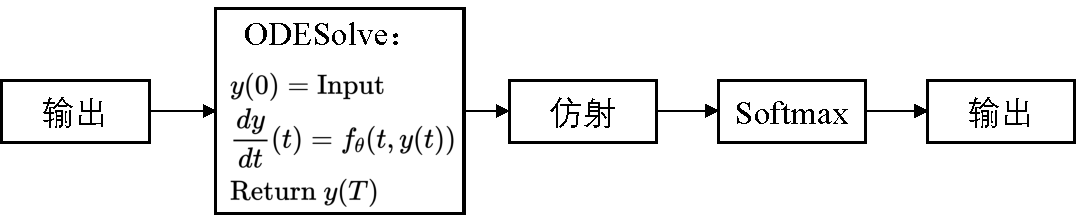
\includegraphics[width=0.9\linewidth]{figures/chapter1/simple_ode.pdf}
    \caption{神经常微分方程的计算图}
    \label{fig:neural_ode}
\end{figure}

ODE-Net的主要应用包括Res-Net的替代、时间序列建模以及可逆正则化流\cite{Grathwohl2019}。本文主要围绕ODE-Net在时间序列建模及系统辨识中的应用展开研究。
因为ODE-Net的连续时间特性,该方法能够将深度网络模型应用于连续时间域下的时间序列建模问题研究中,开辟了时间序列分析、连续时间系统建模研究的新思路。
% 接下来本节将简单介绍几种常见的微分方程网络及其应用。

在处理时间序列问题时,相比于RNN等离散时间步下的循环神经网络。ODE-Net天然地适用于建模非均匀采样的时间序列。如基于ODE-Net衍生的ODE-RNN\cite{10.5555/3454287.3454765}、GRU-ODE-Bayes\cite{brouwer2019gru}、ODE-LSTM\cite{lechner2020learning}。
为了求解ODE-Net的初值,Latent ODE\cite{10.5555/3454287.3454765}将ODE-Net的初始状态视为先验分布为标准高斯分布的因变量,利用编码器-解码器结构实现序列的重构、插值、预测,并使用变分贝叶斯方法对模型进行训练。
文献\cite{Yildiz2019}基于贝叶斯理论,构建了2阶ODE-Net模型用于高维时间序列的建模,同时利用ODE-Net连续正则化流的特性估计待预测时间点隐变量的后验分布并引入分布正则化对隐状态的范围作出限定。

% \subsection{常微分方程网络}
在常微分方程网络求解器效率的优化方面,
% chen等最早提出常微分方程网络化\cite{chen2018neural}开创了深度学习与微分方程结合的先河。
% 为了加速ODE-Net的求解,
Zhuang等\cite{Zhuang2020}提出了自适应检查点联合状态方法以改进原始联合敏感度法求解梯度的精度以及效率。正则化神经常微分方程(regularized neural ODE,RN-ODE)\cite{J2020}基于理论保证的最优传输和稳定性正则化简化ODE系统,能够有效优化ODE-Net的数值积分求解效率。
除此之外,对ODE方程的高阶导数正则化\cite{kelly2020}对求解时间点添加随机扰动\cite{Ghosh2020}等方案也能够起到正则化作用,加速ODE-Net的求解效率。


% \subsection{受控微分方程网络}
由于常微分方程的解仅由初始状态决定,无法基于后续的观测对轨迹进行调节,使得诸如latent-ode、ODE2VAE等模型将序列观测信息全部压缩至初始状态中,有可能造成观测信息的信息损失。
神经受控微分方程(Neural Controlled Differential Equation)\cite{kidger2020neural}将受控信号的微分项融入在ODE网络的求解中。相比于在求解时间区间的间隔点处利用观测数据对隐状态进行更新的方法(如ODE-RNN、ODE-LSTM等),获得了更好的序列信息提取与表示能力。
为了解决神经受控微分方程在长时间序列场景下难以训练的问题,基于对数签名变换(Log signature transform)的Log-signature/NCDE方法\cite{morrill2021neural}通过签名变换对受控信号进行转换,能够增加模型训练速度、减少存储开销、改进模型预测性能。
针对常规的受控微分方程需要对离散序列进行样条插值,无法实现在线预测的情况,Morrill等\cite{morrill2021online}描述了受控微分方程中连续控制信号应满足的性质,并给出了三次埃尔米特直线插值方法,使受控微分方程网络能够类似于RNN一样,实现在线的时间序列数据处理,而不需要预先对完整的序列数据进行插值。
% \subsection{随机微分方程网络}

在常微分方程网络及受控微分方程网络的基础上,随机微分方程网络相比于常微分方程添加了扩散项(Diffusion process)。
对于随机微分方程的训练也可以采用联合敏感度法(Adjoint Sensitibity)进行训练\cite{li2020scalable}。由于随机微分方程网络的前向传播过程依赖于带有随机性的Wiener过程,为了避免存储完整的计算图,需要保证反向求解SDE时对Wiener过程的采样与前向传播保持一致。文献\cite{li2020scalable}利用基于虚拟布朗树(Virtual Brownian Tree)的伪随机数生成策略,仅需常数级存储$\mathcal{O}(1)$即可对的SDE网络前向传播的Wiener过程采样结果进行存储。节约存储空间的代价为对特定时间点下的wiener过程采样时间复杂度为$\mathcal{O}(\log n)$。
将微分方程网络作为Res-Net的替代品处理图像领域问题时,有研究表明将ODE-Net替代为SDE-Net,在ODE-Net中增加随机扩散项,也能够起到随机正则化的作用,提升网络的泛化能力\cite{Oganesyan2020}。
神经跳变随机微分方程(Neural Jump Stochastic Differential Equations,NJSDE)\cite{Jia2019}将扩散项中对时间的微分替换为观测点次数的微分,能够在建模系统隐空间连续时间动态的同时对观测点出现事件本身以及时刻进行建模,该模型有效地应用于地震预测及药物预测。

% \subsection{受控微分方程网络}
% \section{深度微分方程网络的应用}
% \subsection{}
% ODE-Net作为Res-Net的替代,可以应用于图像处理问题中:如图像超分问题\cite{OISR,jia2019focnet}。
在系统辨识领域,
在许多真实的工业场景中,从被识别系统采样得到的序列数据经常是间隔非均匀的。利用微分方程网络模型能够有效建模系统输出或隐空间状态在外部输入影响下的瞬时变化。
Zhong等\cite{zhong2019symplectic}采用ODE-Net对符合哈密尔顿特性的动态系统进行建模学习,巧妙地将物理先验知识融入到学习模型的设计中。并有效地应用于符合哈密尔顿性质的刚体系统建模与控制问题中。
Ayed等\cite{ayed2019learning}采用ODE-Net模型从系统状态的部分可观测信息学习复杂非线性时空过程。该方法有效应用于水流动预测、Navier Stokes方程、海洋温度分析。
% SNODE\cite{Quaglino2019}模型基于勒让德多项式构建ODE-Nets的压缩表示并应用于系统辨识。
SNODE\cite{Quaglino2019}使用谱方法用于快速和准确地训练神经常微分方程模型以辨识低维输入输出系统。
ODE-RNN~\cite{Rubanova2019}在RNN网络相邻状态更新处插入ODE-Net模块,用于建模网络隐状态的连续时间演化。
为了改善辨识模型在长期预测时的稳定性,如本文第三章所述的稳定性模型,现有研究\cite{Demeester2019,Yuan2022}将递归神经网络的稳定性融入到微分方程的导数网络设计中以解决单位根问题,并提出了一种连续时间系统辨识模型——时间感知的RNN模型。

为了建模来自于多智能体系统的非均匀采样数据,LG-ODE模型\cite{Huang2020}将图神经网络、自注意力以及ODE-Net进行结合,利用时序自注意力模型构建微分方程求解的初态,采用图神经网络建模观测点的时序依赖关系和不同观测项之间的空间依赖关系,并以此为基础估计常微分方程中的隐状态导数。模型有效地应用于稀疏序列的插值预测与外推预测。


对于Transformer、AttentionSeq2Seq等基于注意力的序列处理模型,利用ODE-Net的连续时间特性可以构建连续时间注意力模型\cite{chen2021continuous},并将注意力机制应用于非均匀采样的时间序列。
近年来,Transformer模型\cite{Vaswani2017}因在序列数据处理问题上的优异表现受到了学者的广泛关注,基于Transformer的长序列预测模型,如Informer\cite{Zhou2020}、Autoformer\cite{Wu2021}等均获得比传统时序预测算法更优的预测精度。
得益于ODE-Net的连续时间特性,该模型能够与Transformer进行结合,处理非均匀采样数据或长序列预测及建模问题,如构建连续时间注意力\cite{chen2021continuous}、辅助位置编码(position embedding)\cite{Liu2020}。
正因为ODE-Net模型能够利用非均匀采样数据拟合动态系统,因此可用于有模型强化学习\cite{Yildiz2021}领域,构建可微分的系统状态演化估计器,进而辅助策略模块的学习。
对于系统动态已知的连续时间系统,利用ODE-Net可以为策略网络构建连续时间梯度估计器\cite{Ainsworth2020},使控制和仿真任务的学习更高效、更鲁棒。

\subsection{系统长时延特性建模}
近年来,Transformer模型\cite{Vaswani2017}因在序列数据处理问题上的优异表现受到了学者的广泛关注,基于Transformer的长序列预测模型,如Informer\cite{Zhou2020}、Autoformer\cite{Wu2021}等均获得比传统时序预测算法更优的预测精度。
对于Transformer、AttentionSeq2Seq等基于注意力的序列处理模型,利用ODE-Net的连续时间特性可以构建连续时间注意力模型\cite{chen2021continuous},并将注意力机制应用于非均匀采样的时间序列。

得益于ODE-Net的连续时间特性,该模型能够与Transformer进行结合,处理非均匀采样数据或长序列预测及建模问题,如构建连续时间注意力\cite{chen2021continuous}、辅助位置编码(position embedding)\cite{Liu2020}。
\subsection{跳变系统辨识}
连续时间跳变系统包含多个连续时间子系统,且受到隶属有限状态集的内部阶段变量控制\cite{8709809}。
以最简单的连续时间跳变线性系统\cite{fang2002stabilization}为例:
\begin{equation}
    \dot{x}(t)=A(\sigma(t)) x(t)+B(\sigma(t)) u(t)
\end{equation}
% In order to learn the CTJS from available data, previous studies have assumed the prior structures of system and employed methods such as EM algorithm\cite{balenzuela2022parameter}, Sequential Monte Carlo (SMC)\cite{6859280}, and variational inference \cite{opper2007variational} to estimate the ``grey-box'' model parameters.
$A$和$B$为模型参数。
$\sigma(t)$为有限状态随机跳变过程,通常表示为时间自治的、状态有限的马尔科夫过程。

定义状态集$\underline{N}=\{1,2, \ldots, N\}$,对于所有 $i, j \in \underline{N}$,定义状态转移概率矩阵:
\begin{equation}
    \begin{aligned}
    &p_{i i}=0\\
    &q_i=-q_{i i}=\sum_{l \neq i} q_{i l}\\
    &p_{i j}=\frac{q_{i j}}{q_i}, \quad(i \neq j) .
    \end{aligned}
\end{equation}

给定单步转移概率矩阵为$\left(p_{i j}\right)_{N \times N}$,$\left\{r_k ; k=1,2, \ldots\right\}$表示离散时间马尔科夫链,也成为连续时间阶段信号$\{\sigma(t)\}$的嵌入马尔科夫链。相邻跳跃之间的滞留时间用$\tau_k$表示,初始状态表示为$\sigma (0)=i$。过程以概率$p_{ij}$跳跃至状态$j\neq i$,在阶段$j$下的滞留时间服从参数为$q_i$的指数分布。
过程$\{\sigma(t)\}$访问过的状态表示为嵌入马尔科夫链$\left\{r_k ; k=1,2, \ldots\right\}$,相应的滞留时间$\left\{\tau^{\left(r_k\right)}\right\}$是服从独立指数分布的随机变量,分布参数为$q_{i_k}$。
联合过程$\left\{\left(r_k, \tau_k\right): k=0,1, \ldots\right\}$是时间同质的马尔科夫过程,完全确定了跳变系统阶段变量$\{\sigma(t)\}$。

为了从包含多阶段混合数据的离线序列中学习连续时间跳变系统参数$\{A(i),B(i);i \in \underline{N}\}$以及阶段切换参数$\{q_i,p_{ij};i,j \in \underline{N}\}$,Ashley等采用序列蒙特卡洛(Sequential Monte Carlo, SMC)\cite{ashley2014sequential}将辨识问题转换为一般的非线性状态空间估计问题。不过该方法计算量较大。
为了更有效地利用有限的计算资源,随机近似(Stochastic approximation, SA)\cite{svensson2014identification}思想被引入SMC框架中。变分近似方法\cite{opper2007variational}是其中的典型代表。

Balenzuela等提出了一种基于EM算法的马尔科夫跳变系统辨识方法\cite{balenzuela2022parameter}。
为了克服传统方法中E步计算复杂度随阶段数指数增长的问题,该文章提出的EM方法在合并高斯成分的E步内使用近似算法,以减少高斯分量的数量。
原则上,该方法不需要SMC和随机逼近方法中通常需要的渐近参数,就可以得到精确解。

Opper等\cite{opper2007variational}提出采用平均场理论,在给定有噪音的观测数据下,近似推理阶段变量以及估计系统参数。相比于马尔科夫链蒙特卡洛(Markov chain Monte Carlo, MCMC)方法关注于在阶段转换发生时从局部时间范围内进行采样,该方法计算系统可能转移路径的概率分布的近似,因而易于实现平均场的因子化。

\subsection{动态系统随机非确定性的表示与推理}
现有的大部分连续时间模型能够有效解决系统的不均匀采样问题,但由于其模型内部状态的转换是确定性的,因此对于存在随机性的系统,其建模能力较弱。
在建模随机性系统方面,深度时序生成模型~\cite{Fraccaro2016,Chung2015,Karl2017},一般也称谓深度状态空间模型(Deep State Space Model, Dssm)将变分自动编码器模型(Variational Auto-encoder)~\cite{kingma2013auto}扩展到了序列数据。

此类模型通过引入时序的随机隐变量学习序列的随机性。
类似地,PR-SSM~\cite{doerr2018probabilistic}和PILCO~\cite{deisenroth2011pilco}采用高斯过程来学习输入/输出系统的概率状态空间模型。

利用上述方法构建的序列生成模型能够极为便捷地在给定条件序列输入的情况下,预测输出分布并从中采样。这种性质也使得这些方法广泛应用于缺失数据填充\cite{Fraccaro2017}、开环预测\cite{Hafner2019}、基于模型的强化学习等任务\cite{Hafner2019}。

以往的一些工作尝试将时序变分推理框架与微分方程网络相结合,用于学习随机的连续时间过程处理非均匀采样的序列数据。
LatentODE\cite{Rubanova2019}、 ODE2VAE\cite{Yildiz2019} 和 LatentSDE\cite{Li2020}利用非均匀观测数据推理隐状态的近似后验分布。
通过从近似后验中采样状态并求解参数化的微分方程网络,模型能够从连续时间域角度对给定时间区间上的任一点进行插值或预测,进而有效地解决非均匀采样观测下的随机系统预测问题。

然而,由于这些模型在预测或插值前必须输入完整的采样序列以用于隐状态的推理,因此这些模型均是离线模型\cite{Liu2020}。
在某些特定任务中,如本文关注的在线控制,预测模型需要能够运行在在线模式下以处理流式数据。如循环神经网络,可以支持递归地输入单点数据并更新其内部状态。


\section{本章小结}
从上述文献可以发现,因微分方程网络所具备的连续时间特性,
此类模型广泛应用于时间序列分析、时间点过程分析、连续时间动态系统识别等问题,并有效支撑了时序预测、稀疏序列插值、系统控制等应用任务。目前为止,基于微分方程网络的动态系统识别方法尚在研究初期,如何面向不同类型的复杂动态系统选择合适的网络结构以及模型训练方法是该领域尚待解决的关键问题。
